Version 1 largely adheres to the design specification.

\begin{figure}
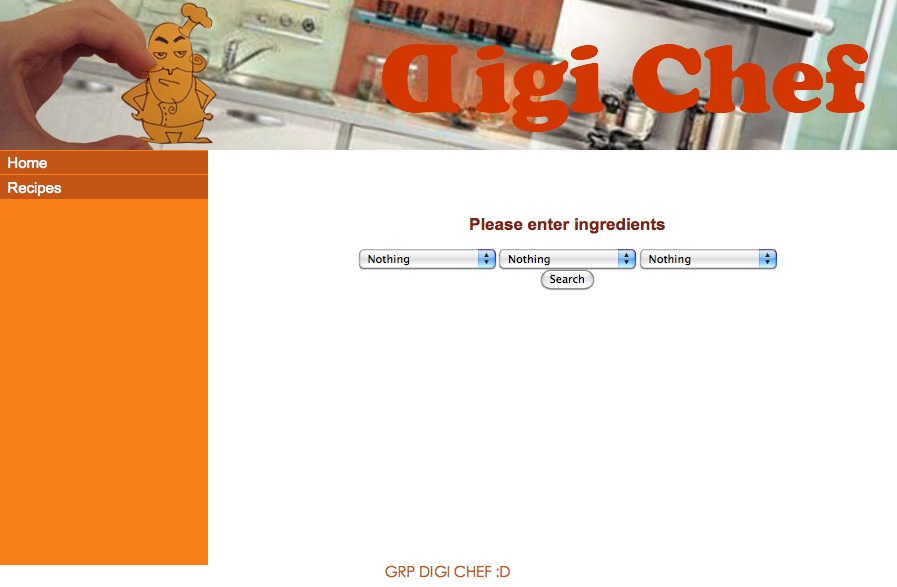
\includegraphics[width=0.9\textwidth]{result_1}
\caption{Homepage}
\label{fig:result_1}
\end{figure}


As mentioned, white and orange are the colours of choice, along with an appealing logo. The design is simple and effective in meeting the needs of version 1.(Fig~\ref{fig:result_1}) shows the drop down menus for ingredient selection with the search option.

(Fig~\ref{fig:result_2}) shows the result of ingredient selection by the user. The recipe list was generated based on the ingredients selected by the user.

\begin{figure}
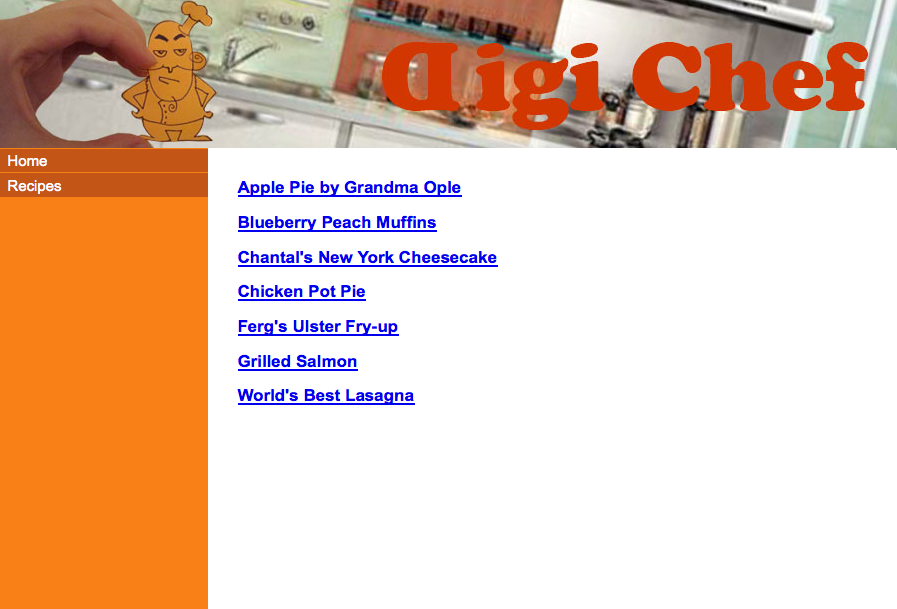
\includegraphics[width=0.9\textwidth]{result_2}
\caption{Search results}
\label{fig:result_2}
\end{figure}

(Fig~\ref{fig:result_3}) shows the result of clicking on a recipe. Notice the Recipes button on the far left hand side of the web page. Clicking that generates the list of all recipes in the database.

\begin{figure}
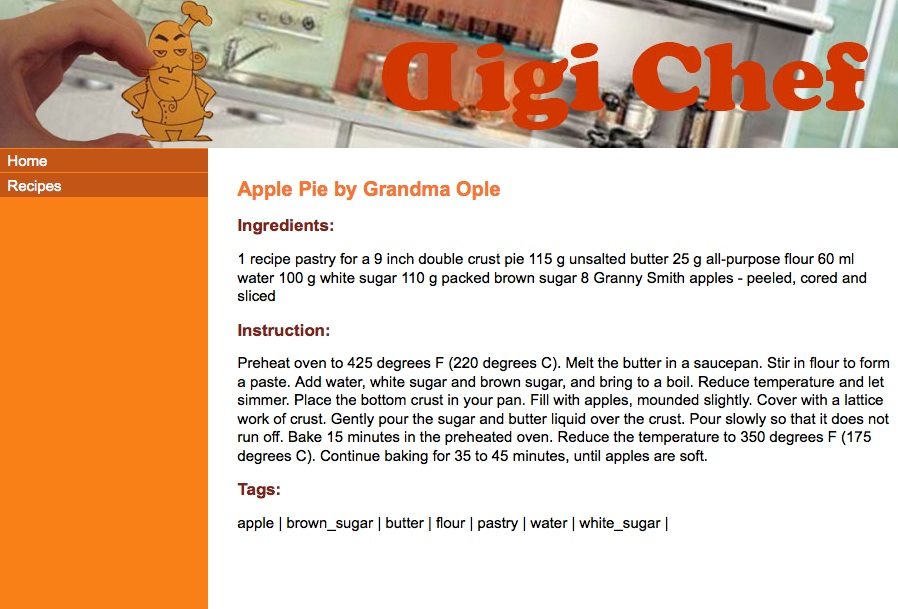
\includegraphics[width=0.9\textwidth]{result_3}
\caption{Recipe page}
\label{fig:result_3}
\end{figure}

The group thoroughly scoured the website of bugs by doing exhaustive testing of all the possible ingredients and checking if the returned list matches the input ingredients. Exhaustive testing was possible for version 1 due to the small database and only three ingredient boxes. However, as our system gets more complicated, this form of testing will be unwieldy. A better method of testing will be required then.

